%% \subsubsection{Changing the overall shape and stress range}
%% \label{changing-shape}

%% \textbullet\ All the plots shown thus far have had the same general
%% shape, but experiments show different things for different tissues at
%% different ages. We can easily model this by changing the material
%% parameters to change the stress-ranges and shapes.

%% \begin{figure}[!hptb]
%% \centering
%% \includegraphics[width=0.6\textwidth,angle=270]{images/examples/%
%% eulerian/pulling/plots/poro-elastic/low-hysteresis-dynamic-0p01-d1p037}
%% \caption{Dynamic poroelastic model, $\dot{\epsilon}=0.01$ Hz, $D=1.037$
%%   MPa.s.mm$^{-2}$.}
%% \label{low-hysteresis-dynamic-0p01-d1p037}
%% \end{figure}

%% \begin{figure}[!hptb]
%% \centering
%% 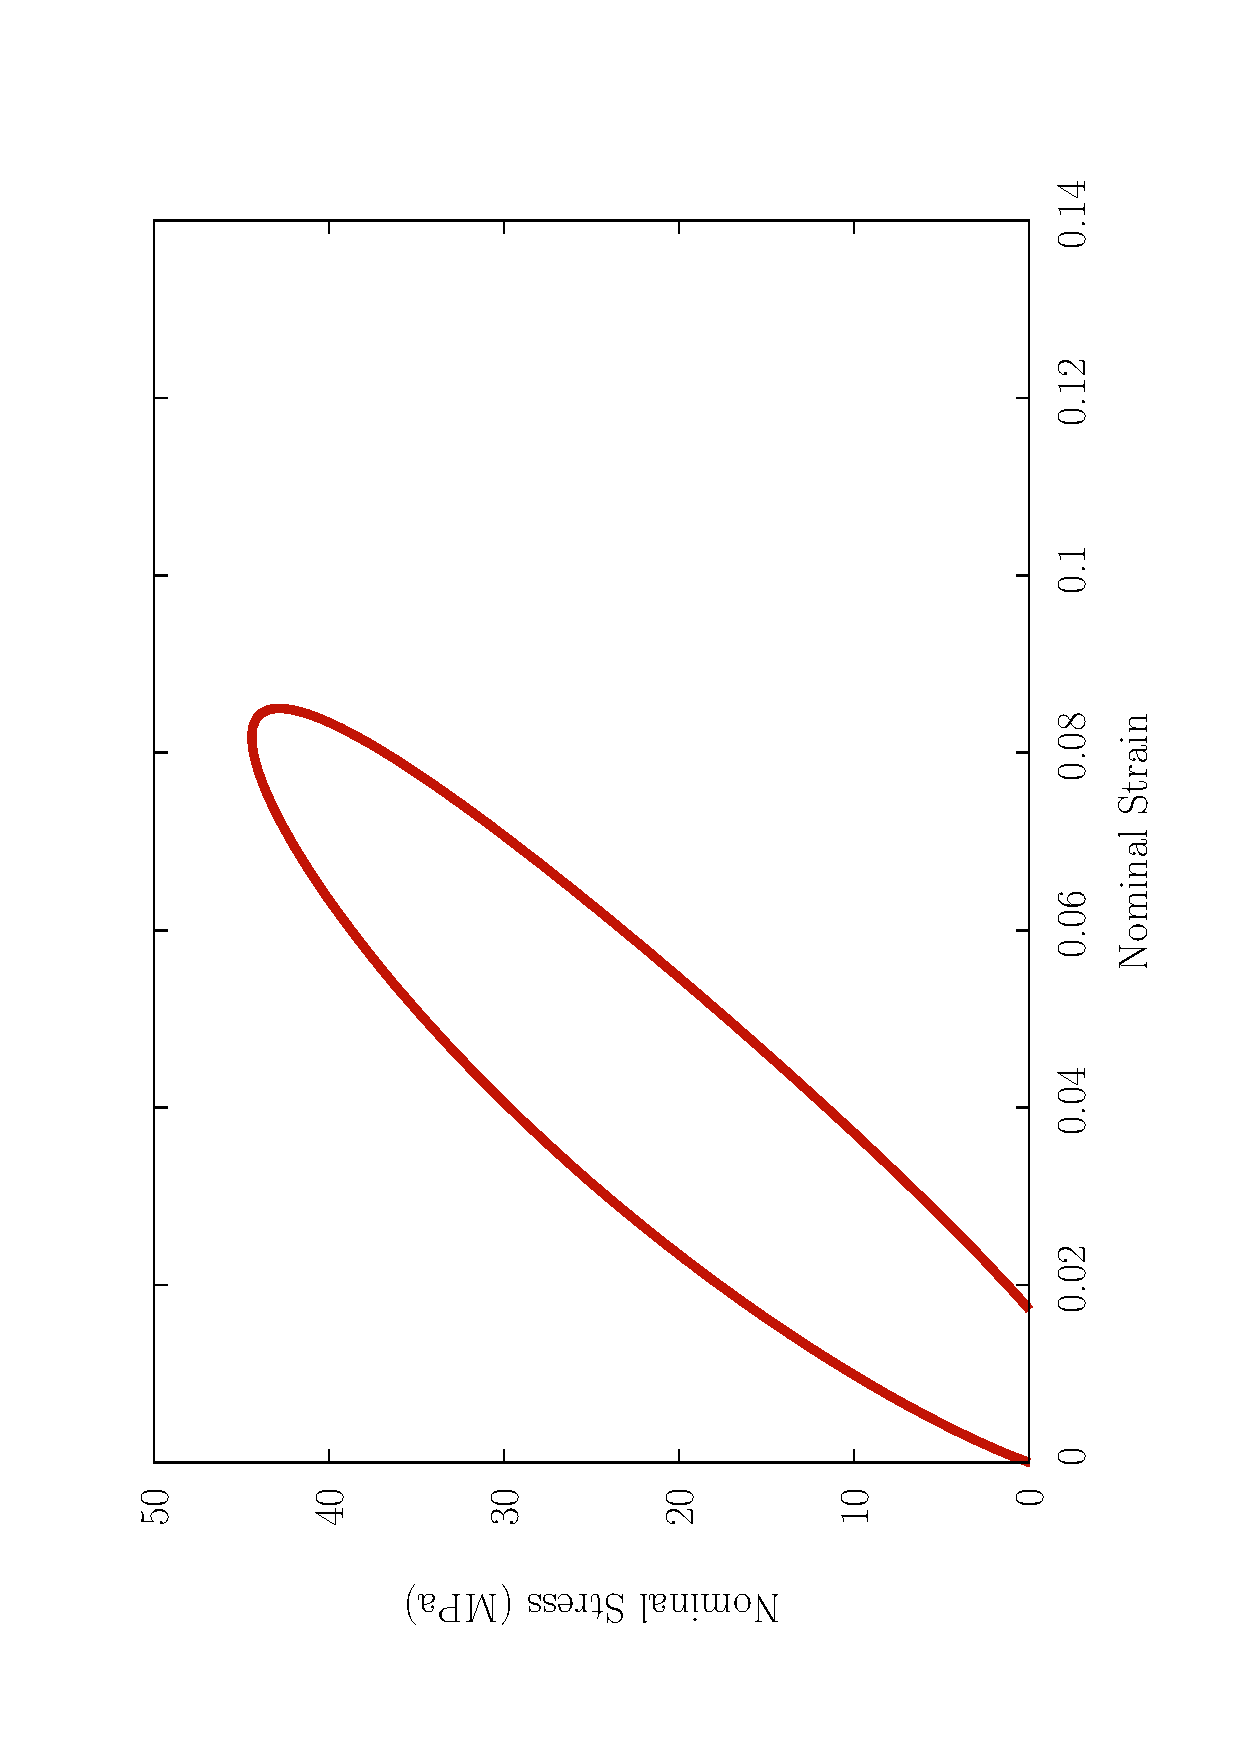
\includegraphics[width=0.6\textwidth,angle=270]{images/examples/%
%% eulerian/pulling/plots/visco-elastic/low-hysteresis-visco-0p01-t0p7}
%% \caption{Dynamic viscoelastic model, $\dot{\epsilon}=0.01$ Hz,
%%   $\tau=0.7$ s.}
%% \label{low-hysteresis-visco-0p01-t0p7}
%% \end{figure}

%\subsection{Flow fields under tension}
%\label{tension-flow} -- Can be moved in with the tension tests
